\appendix
\section{Esquemáticos dos circuitos}

\subsection{Planta em malha aberta}

\begin{figure}[H]\label{ltspice:ol} 
\begin{center}
    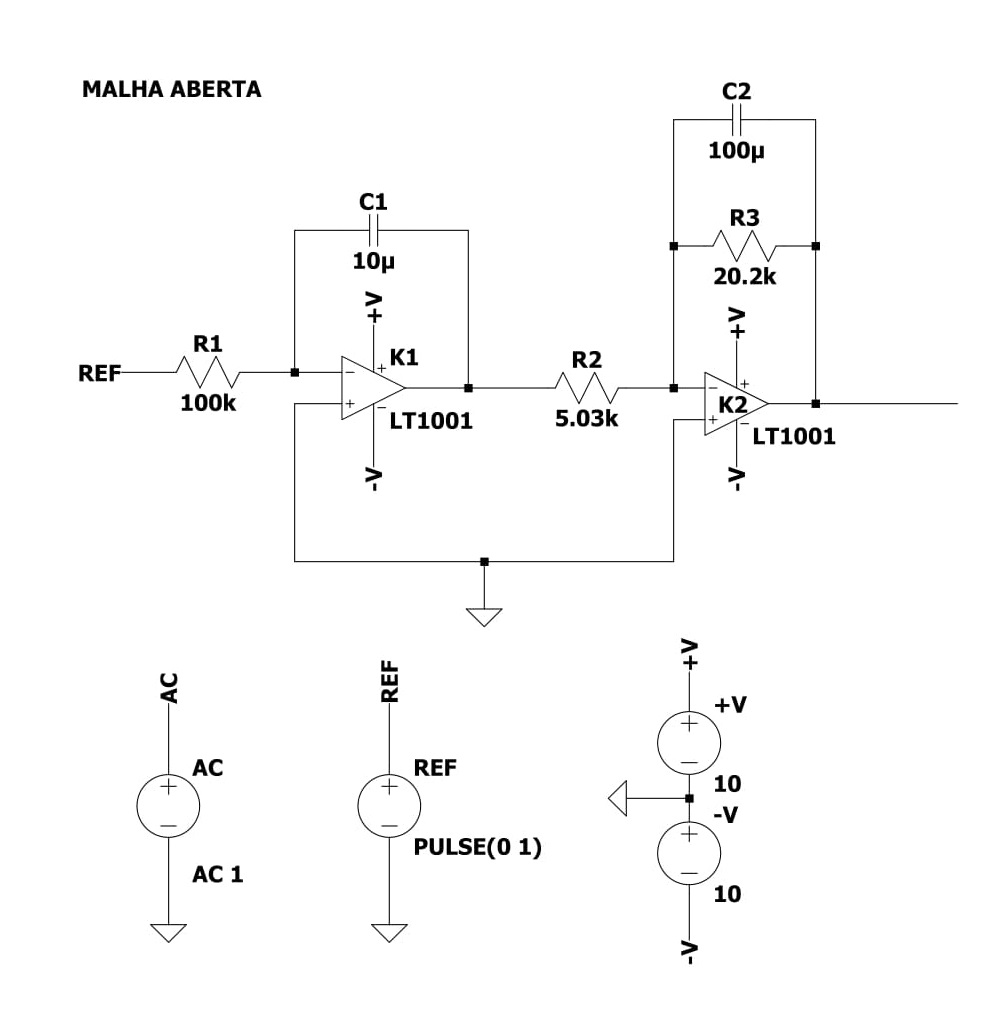
\includegraphics[scale=0.5]{images/PD_pratico/ol_ltspice.jpg}  
\end{center}
%\label{ltspice:ol} 
\end{figure}

\subsection{Planta em malha fechada}

\begin{figure}[H]\label{ltspice:cl} 
\begin{center}
    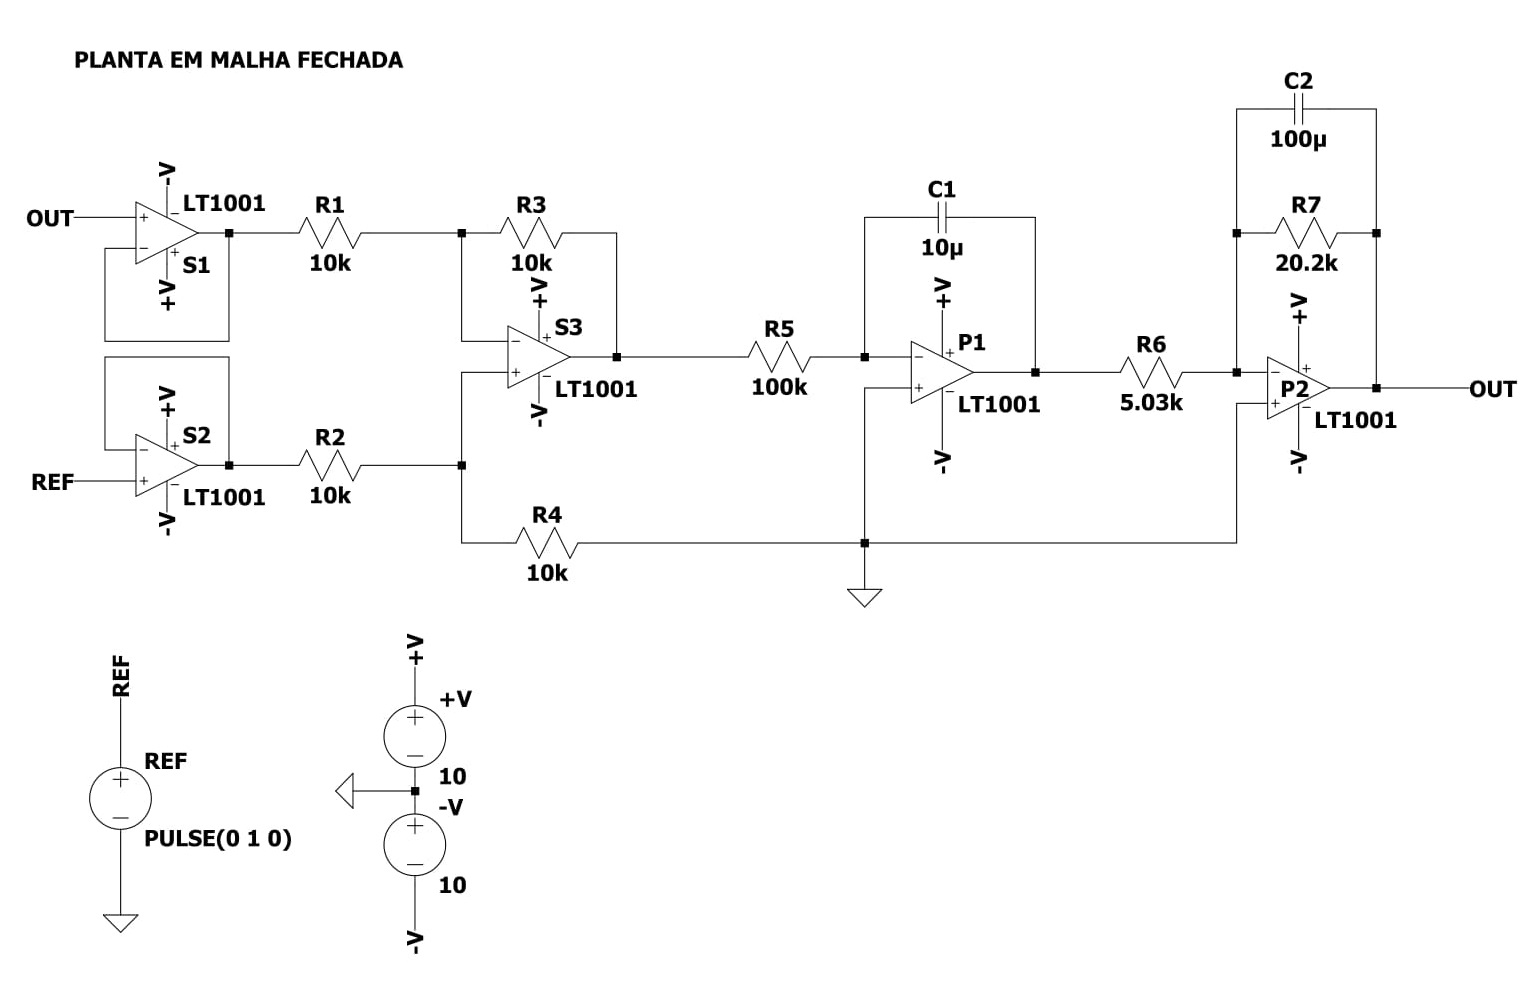
\includegraphics[scale=0.4]{images/PD_pratico/cl_ltspice.jpg} 
\end{center}

%\label{ltspice:cl} 
\end{figure}

\subsection{Planta e controlador PD em malha fechada}

\begin{figure}[H]\label{ltspice:clpd} 
\begin{center}
    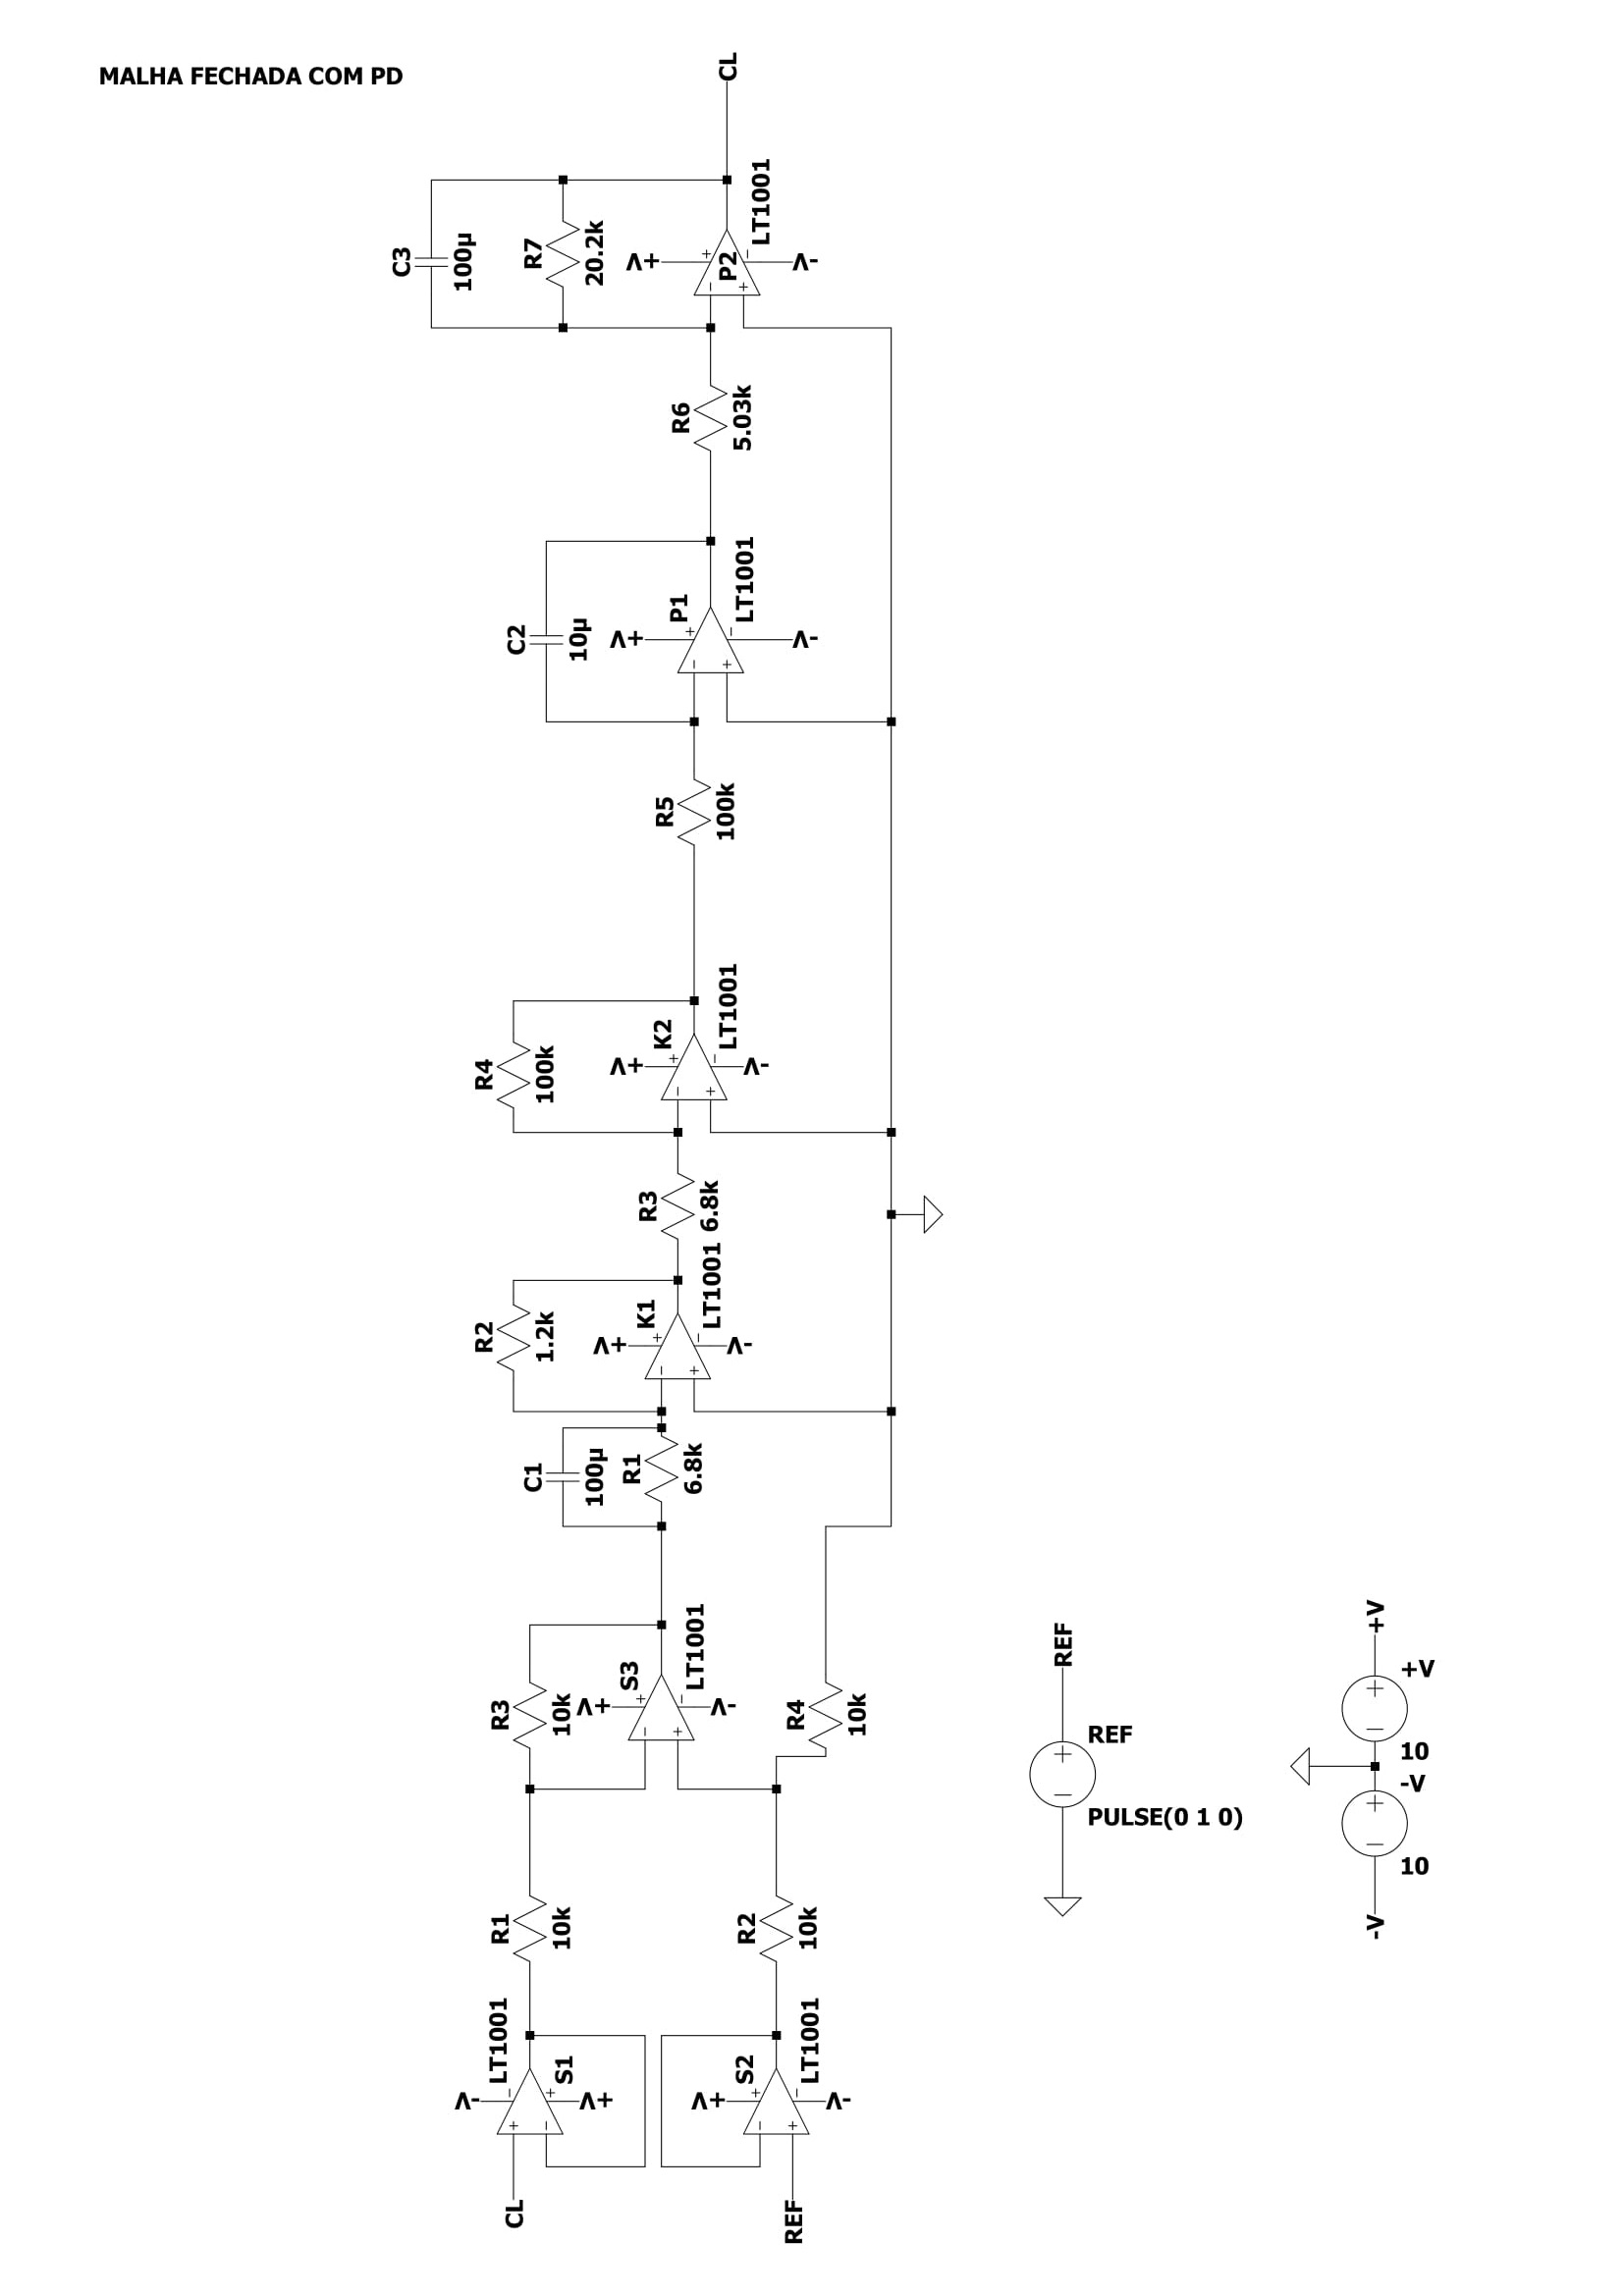
\includegraphics[scale=0.33]{images/PD_pratico/cl_pd_ltspice.jpg}  
\end{center}
%\label{ltspice:clpd} 
\end{figure}

\pagebreak

\section{Scilab \textit{scripts}}

\subsection{Margens de estabilidade e diagramas de Bode e Nyquist}

\begin{lstlisting} 
limit = 10000;
s = poly(0, "s");
//planta
P = syslin('c', 2/(s*(s+0.5)));
//planta+PD
P_PD = syslin('c', 2.4271*(1+0.573302*s)*2/(s*(s+0.5)));

//plots de Bode e Nyquist
figure;
bode(P);
xname("Diagramas de Bode da planta")
figure;
nyquist(P);
xname("Diagrama de Nyquist da planta")
figure;
bode(P_PD);
xname("Diagramas de Bode da planta com PD")
figure;
nyquist(P_PD);
xname("Diagrama de Nyquist da planta com PD")

// margens de estabilidade
[MF_p, fcg_p] = p_margin(P);
[MG_p, fcf_p] = g_margin(P);
fcg_p = 2*%pi*fcg_p;
fcf_p = 2*%pi*fcf_p;
[MF_ppd, fcg_ppd] = p_margin(P_PD);
[MG_ppd, fcf_ppd] = g_margin(P_PD);
fcg_ppd = 2*%pi*fcg_ppd;
fcf_ppd = 2*%pi*fcf_ppd;

\end{lstlisting}


